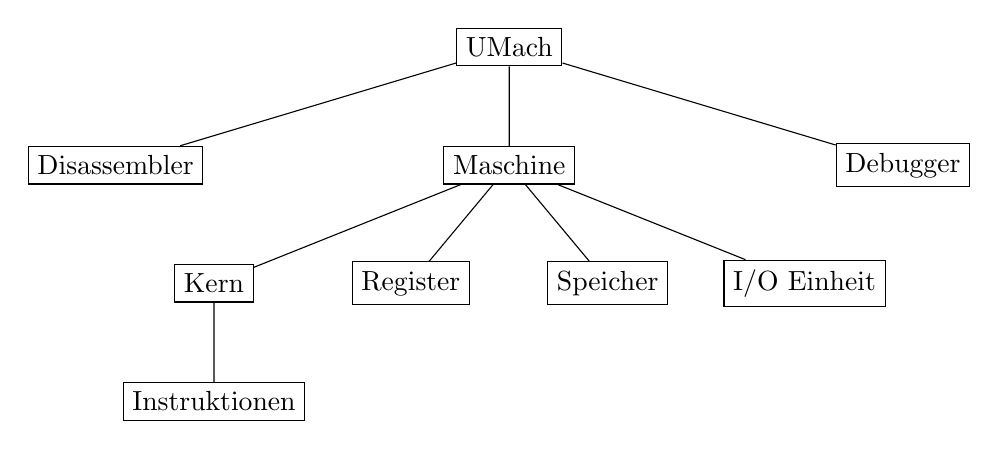
\begin{tikzpicture}
[every node/.style={draw},
 level/.style={sibling distance=5cm/#1}]
\node{UMach}
child
{
    node {Disassembler}
}
child 
{
    node {Maschine}
    child
    { node{Kern}
      child { node{Instruktionen} }
    }
    child { node{Register} }
    child { node{Speicher} }
    child { node{I/O Einheit} }
}
child
{
    node {Debugger}
}
;
\end{tikzpicture}
 
